\subsection{《满汉文化交融视野下的红楼梦研究》}

\subsubsection{读后感}
这是山东大学白燕的博士论文,从清代中前期北京满人文化为切入点分析了《红楼梦》中的满人习俗和文化,认为《红楼梦》是满汉文化交织下的文学巨著。 

从我个人而言,之前读周汝昌等人的著作,似乎并未着重强调满人习俗。经过阅读此论文,对《红楼梦》的产生有了更全面的认识。本文论据基本上很有说服力,结论是可靠的。不过,一些细节论证,比如一些满人习俗是否为满人所独有,是存疑的。

\subsubsection{摘抄}
曹家这种既是奴仆又是显贵的双重身份,既卑贱又显赫的矛盾心理,以及主仆之间微妙复杂的情感纠结,对曹雪芹的思想产生了极大的影响。 

曹雪芹在作品中所表达的忠君思想,既是对中国两千多年来自汉代完整定型的三纲五常思想的继承,同时又具有满族的对长上特别是对君王绝对忠诚的特色。在八旗社会,所有的八旗军民士庶在皇帝面前一律自称奴才,而称皇帝为主子。太田辰夫曾将八旗精神的中心概括为是对清朝廷的忠诚。 

戴震的批判目标非常明确,即程朱理学,是从儒学内部起来批判正统理学而曹雪芹则把目标直接对准了儒家礼法。……戴震指出,理是日用人伦生生之事的规范,欲是与生俱来的自然属性因此理就得本之于生养之情欲去求,唯有情欲不爽失才是理理在情欲之中,离开了情欲也就无所谓理人我情欲皆得遂顺,才是理。 

(清易易服剪发)生必从时服,死虽古服无禁;成童以上皆时服,而幼孩古服亦不禁;男子从时服,女子犹袭明服。盖自顺治以至宣统,皆然也。 

(贾宝玉在家梳头的发式)四周梳小辫,归至顶心编成大辫,这是满洲子弟幼年的发式。 

红楼梦中涉及的满洲发式服饰食物:
\begin{itemize*}
	\item 辫发
	\item 留头
	\item 杩子盖
	\item 满族头饰
	\item 袍子
	\item 褂子
	\item 箭袖
	\item 鹰膀
	\item 八团
	\item 靴
	\item 荷包
	\item 如意
	\item 满洲饽饽
	\item 野味
	\item 女子天足
	\item 女子吸烟(一零一回凤姐)
	\item 兽皮
\end{itemize*}
红楼梦中的满洲称谓:
\begin{itemize*}
	\item 老祖宗
	\item 爷,奶奶
	\item 哥儿
	\item 姐儿,姑娘
	\item 妞妞
	\item 哥哥,姐姐,满洲世家常日称呼嫂子为”姐姐“
	\item 家的
	\item 嬷嬷
	\item 主子,奴才
\end{itemize*}
《红楼梦》中的婚姻、丧葬习俗也有满人的影子,比如夜婚,助哭等。另外,极度讲究尊卑、重视女性、请安、以西为上、祭祀用品、跳大神、放鹰、玩鸟儿等习俗也是满礼。

清朝建国八公皆国初有大勋劳者,世袭不降封:
\begin{itemize*}
	\item 礼亲王代善
	\item 郑亲王济尔哈朗
	\item 睿亲王多尔衮
	\item 豫亲王多铎
	\item 肃亲王豪格
	\item 敬谨亲王尼堪
	\item 克勤郡王岳讬
	\item 顺承郡王勒克德浑 
\end{itemize*}
	另外还有四个亲王世袭罔替:
\begin{itemize*}
	\item 怡亲王允祥
	\item 恭亲王奕
	\item 醇亲王奕繯
	\item 庆亲王奕劻
\end{itemize*}

清朝皇家拿奴才管天下的思路,确实让汉族士人压抑。清朝文化之沉闷,远失汉人挥斥天下的风采。

清朝官员的俸禄:
\begin{figure}[htpb]
\centering
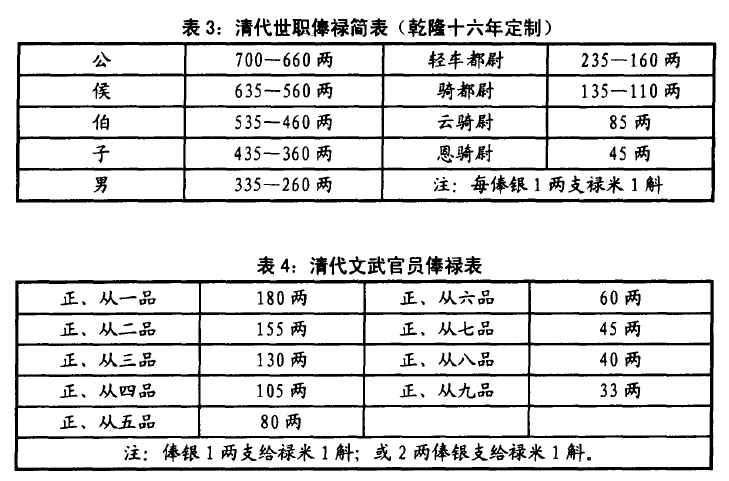
\includegraphics[width=0.5\linewidth]{images/fenglu.png}
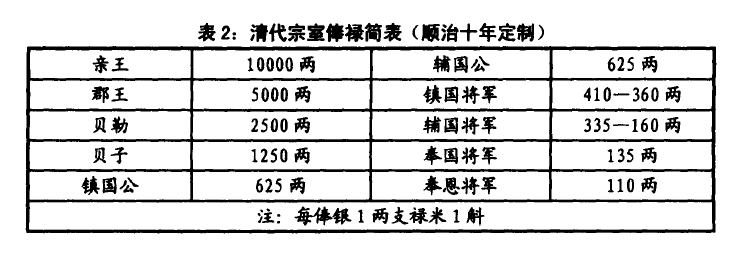
\includegraphics[width=0.5\linewidth]{images/fenglu2.png}
\end{figure}

曹雪芹进步妇女观的形成,既受明中叶以来的时代进步思潮影响,更与满族社会特殊的妇女地位有关。 

相对而言,清代八旗世家对封建礼法的恪守远甚于当时的汉族世家。 

旗人社会中的女子持家、重小姑、重内亲等习俗在《红楼梦》中都有生动体现

清代的满族贵族文化,是中国历史上在官僚社会中唯一形成了自己特色的贵族文化。 
“有闲性”是京旗文化的显著特征,并构成了与中国历史上影响深远的士文化的重要区别。 

最早的《三国志演义》还是半文半白,《水浒传》、《金瓶梅》使用的是山东方言,《西游记》、《儒林外史》用的则是长江流域官话,到《红楼梦》才真正开始使用北京话写作。 

《红楼梦》中不仅出现了“克什(恩赐)”、,'海龙(水獭)”、,'妞妞(女孩)“等满语词,而且满式汉语句俯拾即是,如“把莺儿不理”(第三十五回)、“何曾不是在房里来着”(第二十八回)、“将来只怕比这更奇怪的笑话儿还有呢”(第三回)、“要去不能”(第十九回)等,皆有满语语法的痕迹。 

内府包衣由于长期与满洲相处,潜移默化,姓氏逐渐满族化。姓氏满洲化是指放弃自己的汉族姓氏,随同满洲姓氏的特点,即”称名不举姓,人则以其名之第一字称之,若姓然“。

《红楼梦》成书时的传播路径: 
\begin{figure}[htpb]
\centering
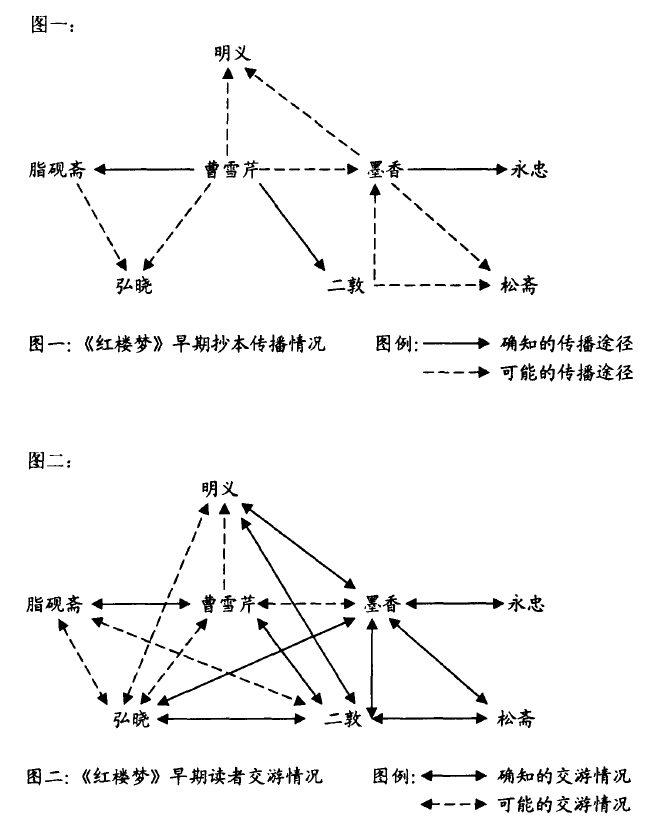
\includegraphics[width=0.5\linewidth]{images/hlmlc.png}
\end{figure}